\documentclass{standalone}
\usepackage{tikz}

\usepackage{ amssymb }
\usetikzlibrary{decorations.pathmorphing}
\usetikzlibrary{arrows.meta}
\usetikzlibrary{arrows}

\begin{document}

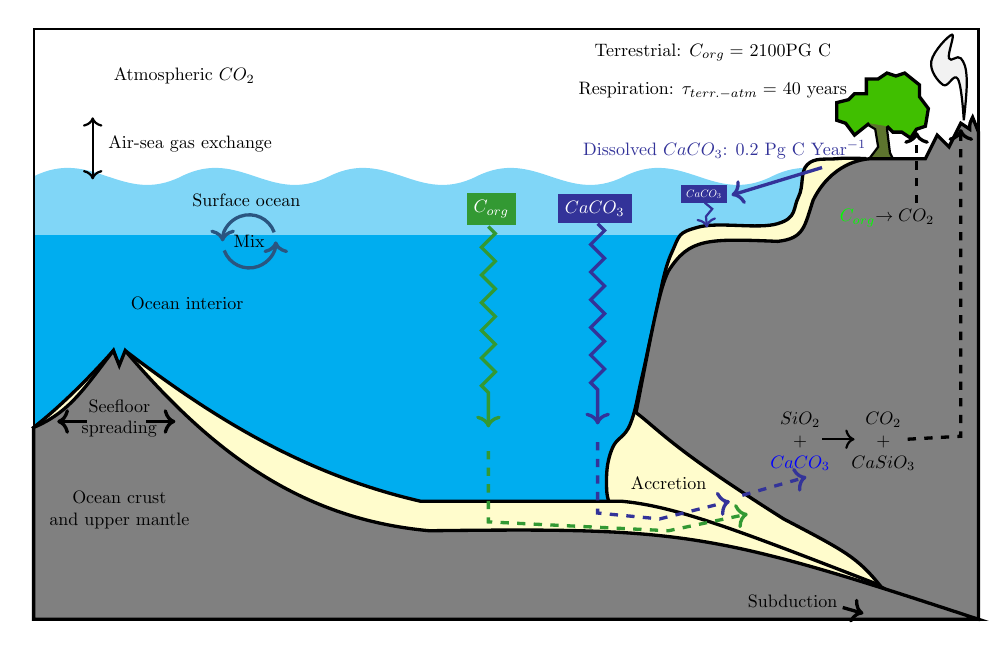
\begin{tikzpicture}[thick,scale=0.75, every node/.style={scale=0.65}]
%\node[style={scale=0.89}] at (-5,5.5) {\includegraphics[width=20.5cm]{Captura2.jpg}};

%mar
\fill[cyan!50] (-13,8) .. controls (-12,8.5) and (-11.5,7.5) .. (-10.5,8) .. controls (-9.5,8.5) and (-9,7.5) .. (-8,8) .. controls (-7,8.5) and (-6.5,7.5) .. (-5.5,8) .. controls (-4.5,8.5) and (-4,7.5) .. (-3,8) .. controls (-2,8.5) and (-1.5,7.5) .. (-0.5,8) .. controls (0.5,8.5) and (1,7.5) .. (2,8) .. controls (1,7) and (1.5,7) .. (0.5,7) .. controls (-5.5,7) and (-7.5,7) .. (-13,7) node (v1) {} .. controls (-13,7.5) and (-13,7.5) .. (-13,8);
\fill[cyan]  (v1) rectangle (2,1.5);
%arbol
\draw [thick,fill={rgb:red,4;green,5;blue,2}](1.55,8.3) -- (1.5,8.4) -- (1.45,8.8) -- (1.5,9) -- (1.45,9.05) -- (1.35,9.05) -- (1.25,9.1) -- (1.2,9) -- (1.1,9.05) -- (1.1,8.95) -- (1,8.95) -- (1.25,8.8) -- (1.3,8.5) -- (1.15,8.3) -- (1.55,8.3);
\draw [very thick,fill={rgb:red,2;green,6;blue,0}](1.45,8.85) -- (1.55,8.75) -- (1.7,8.75) -- (1.85,8.65) -- (1.95,8.8) -- (2.1,8.85) -- (2.15,9.15) -- (2,9.35) -- (2,9.55) -- (1.75,9.75) -- (1.6,9.7) -- (1.45,9.75) -- (1.3,9.65) -- (1.1,9.65) -- (1.1,9.4) -- (0.9,9.4) -- (0.8,9.3) -- (0.6,9.25) -- (0.6,8.95) -- (0.75,8.9) -- (0.9,8.7) -- (1.15,8.9);

%tierra
\draw[very thick,fill=yellow!20]  plot[smooth, tension=.7] coordinates {(1.1,8.3) (0.6,8.3) (0.1,8.2) (-0.05,7.65) (-0.4,7.2) (-1.75,7.14) (-2.2,6.7) (-2.5,5.5) (-2.7,4.6) (-2.9,3.8) (-3.2,3.4) (-3.3,2.85) (-3.2,2.4) (-2.8,2.3) (1.35,1)};
\draw [very thick,fill=yellow!20](-11.45,5.05) .. controls (-9.95,3.9) and (-8.4,2.95) .. (-6.45,2.5) .. controls (-5.25,2.5) and (-4.75,2.5) .. (-3.05,2.5) .. controls (-1.95,2.4) and (-0.7,1.85) .. (2.7,0.55) .. controls (2.7,0.55) and (-11.05,0.55) .. (-11.05,0.55);
\draw [very thick,fill=yellow!20](-11.55,4.75) .. controls (-11.55,4.75) and (-11.65,5.05) .. (-11.65,5.05) .. controls (-12.05,4.6) and (-12.55,4.1) .. (-13,3.75) .. controls (-13,3.75) and (-12.8,3.55) .. (-12.8,3.55);
\draw [very thick,fill=gray!100](1.2,8.3) .. controls (1,8.3) and (0.5,8.2) .. (0.2,7.6) .. controls (0.05,7.15) and (0.05,6.95) .. (-0.4,6.9) .. controls (-1.6,6.95) and (-1.9,6.95) .. (-2.25,6.4) .. controls (-2.4,6.1) and (-2.5,5.55) .. (-2.8,4) .. controls (-2.4,3.7) and (-2.2,3.4) .. (-0.3,2.2) .. controls (0.75,1.65) and (0.95,1.55) .. (1.35,1.05) .. controls (2.05,0.65) and (2.6,0.55) .. (3,0.5) .. controls (3,5.1) and (3,6) .. (3,7.7) .. controls (3,7.95) and (3,7.95) .. (3,8.15) .. controls (3,8.4) and (3,8.45) .. (3,8.75) .. controls (2.9,9) and (3,8.75) .. (2.9,9) .. controls (2.85,8.9) and (2.85,8.9) .. (2.85,8.8) .. controls (2.7,8.9) and (2.85,8.8) .. (2.7,8.9) .. controls (2.6,8.7) and (2.6,8.7) .. (2.5,8.5) .. controls (2.4,8.6) and (2.4,8.6) .. (2.3,8.7) .. controls (2.2,8.5) and (2.2,8.5) .. (2.1,8.3) .. controls (1.9,8.3) and (1.7,8.3) .. (1.2,8.3);
\draw [very thick,fill=gray!100](-13,3.75) .. controls (-12.4,4) and (-12.15,4.4) .. (-11.65,5.05) .. controls (-11.55,4.8) and (-11.65,5.05) .. (-11.55,4.8) .. controls (-11.45,5.05) and (-11.55,4.8) .. (-11.45,5.05) .. controls (-10,3.35) and (-8.5,2.2) .. (-6.3,2) .. controls (-2,2.05) and (-1.55,2) .. (3,0.5) .. controls (-5.6,0.5) and (-5.55,0.5)  .. (-13,0.5) .. controls (-13,3.75) and (-13,0.5) .. (-13,3.75) ;


% otros
\draw  (-13,10.5) rectangle (3,0.5);
%\node at (-10.45,9.7) {Atmosphere: $CO_2=600PgC$};
\node at (-10.45,9.7) {Atmospheric $CO_2$};
\draw [<->](-12,7.95) -- (-12,9);





%\node at (-8.5,8.5) {Air-sea gas exchange: $\tau_{atm-surf.}=$ 7 years};
\node at (-10.35,8.55) {Air-sea gas exchange};
%\node at (-9.15,7.45) {Surface ocean: DIC=700 $\tau_{surf.-deep}=$ 20 years};
\node at (-9.4,7.6) {Surface ocean};
%\node at (-10.4,5.85) {Ocean interior: DIC= 38000PgC};
\node at (-10.4,5.85) {Ocean interior};
%\node at (-8.8,5.35) {$\tau_{deep-surf.}=$ 1000 years};
\node at (-11.55,3.9) {\begin{tabular}{c} Seefloor \\ spreading \end{tabular}};
\draw [->,very thick](-12.1,3.85) -- (-12.6,3.85);
\draw [->,very thick](-11.1,3.85) -- (-10.6,3.85);
\node at (-11.55,2.35) {\begin{tabular}{c} Ocean crust \\ and upper mantle \end{tabular}};
\node at (-1.5,10.1) {Terrestrial: $C_{org}=$ 2100PG C};
\node at (-1.5,9.45) {Respiration: $\tau_{terr.-atm}=$ 40 years};
\node [rectangle,draw={rgb:red,2;green,2;blue,6},fill={rgb:red,2;green,2;blue,6},text=white]  at (-3.5,7.45) {$CaCO_3$};

\node [text={rgb:red,2;green,2;blue,6}] at (-1.3,8.45) {Dissolved $CaCO_3$: 0.2 Pg C Year$^{-1}$ };
\node [rectangle,draw={rgb:red,2;green,6;blue,2},fill={rgb:red,2;green,6;blue,2},text=white] at (-5.25,7.45) {$C_{org}$};
\node [style={scale=0.6},rectangle,draw={rgb:red,2;green,2;blue,6},fill={rgb:red,2;green,2;blue,6},text=white] (v2) at (-1.65,7.7) {$CaCO_3$};
\draw [->,shorten >=-0.3cm,very thick,decorate, decoration={zigzag},draw={rgb:red,2;green,6;blue,2}] (-5.3,7.15) -- (-5.3,4.15);
\draw [->,shorten >=-0.3cm,very thick,decorate, decoration={zigzag},draw={rgb:red,2;green,2;blue,6}] (-3.45,7.2) -- (-3.45,4.2);


\draw[->,shorten >=-0.3cm,very thick,dashed,draw={rgb:red,2;green,6;blue,2}] (-5.3,3.35) -- (-5.3,2.15) -- (-2.25,2) -- (-1.3,2.2);
\draw[->,shorten >=-0.3cm,very thick,dashed,draw={rgb:red,2;green,2;blue,6}] (-3.45,3.5) -- (-3.45,2.3) -- (-2.4,2.2) -- (-1.6,2.4);

\draw[->,shorten >=-0.3cm,very thick,dashed,draw={rgb:red,2;green,2;blue,6}] (-1,2.6) -- (-0.3,2.8);
\draw[->,shorten >=-0.3cm,very thick,draw={rgb:red,2;green,2;blue,6}] (0.35,8.15) -- (-0.8,7.8);
\draw [->,shorten >=-0.3,thick,decorate, decoration={zigzag},draw={rgb:red,2;green,2;blue,6}] (v2) -- (-1.6,7.15);
\draw[->,shorten >=-0.3cm,very thick,dashed](1.95,7.55) -- (1.95,8.35);
\draw[->,shorten >=-0.3cm,very thick,dashed] (1.8,3.55) -- (2.7,3.6) -- (2.7,8.4);
\node at (0.7,3.5) {\begin{tabular}{cc} $SiO_2$ & $CO_2$\\ +&+\\ {\color{blue}$CaCO_3$} & $CaSiO_3$  \end{tabular}};
\node at (1.45,7.3) {{\color{green}$C_{org}$}$\to CO_2$};
\draw[->] (0.35,3.55) -- (0.9,3.55);
\draw[->,very thick,draw={rgb:red,2;green,4;blue,6}]  (-9.7729,6.7461) arc (-160.0028:-0:0.45);
\draw[->,very thick,draw={rgb:red,2;green,4;blue,6}]  (-8.9271,7.0539) arc (19.9972:180:0.45);
\node at (-9.35,6.9) {Mix};
\node at (-0.15,0.8) {Subduction};
\draw[->,very thick] (0.7,0.7) -- (1.05,0.6);
\node at (-2.25,2.8) {Accretion};
\draw[fill=gray!10]  plot[smooth, tension=.7] coordinates {(2.75,8.95) (2.65,9.65) (2.4,9.55) (2.2,9.95) (2.55,10.4) (2.5,10) (2.7,10) (2.8,9.65) (2.75,8.95)};
\end{tikzpicture}
\end{document}